\documentclass[10pt,a4paper]{article}

\setlength{\voffset}{-15mm}
\setlength{\topmargin}{0mm}
\setlength{\headheight}{10pt}
\setlength{\headsep}{5mm}
\setlength{\textheight}{252mm}
\setlength{\textwidth}{170mm}
\setlength{\evensidemargin}{-5.4mm}
\setlength{\oddsidemargin}{-5.4mm}
\setlength{\columnsep}{10mm}
\setlength{\columnseprule}{0.0pt}

%\usepackage[dvipdfm]{graphicx}
\usepackage{graphicx}      % include this line if your document contains figures
\usepackage{amsmath,amssymb}
\usepackage{fancyhdr}
\usepackage{wrapfig}
\usepackage{microtype}
\usepackage{subfig}
\usepackage{caption}
\usepackage{xcolor}
\usepackage{siunitx}

\DeclareMathOperator{\sgn}{sgn}

\newcommand{\bm}[1]{\mbox{\boldmath $ #1 $}}

\makeatletter
   \newcommand{\thefigurename}{Fig.}
   \def \fnum@figure{\thefigurename\ \thefigure}
\makeatother

\captionsetup{width=70mm}
\captionsetup[subfloat]{margin=0pt}
\newcommand{\insfig}[4]{
             \begin{figure}[#3]
             \vspace{-1mm}
             \begin{center}
\includegraphics[scale = #4]{#1}
\end{center}%
             \vspace{-6mm} \hangcaption{#2} \label{#1} \vspace{-2mm}%
             \end{figure}%
             }

\renewcommand{\baselinestretch}{0.95}

%================================================================
\pagestyle{fancyplain}
\lhead{}
\chead{}
\rhead{AVEC '14}
\lfoot{}
\cfoot{}
\rfoot{}
\renewcommand{\headrulewidth}{0pt}

%================================================================
\def\section#1{\refstepcounter{section} \vspace{3.5mm} \noindent
{\normalsize\bf {\thesection.}} \hspace{0.5mm}{\normalsize\bf #1} \par \vspace{2mm}}

%================================================================
\def\subsection#1{\refstepcounter{subsection} \noindent
{\normalsize\bf {\thesubsection}} \hspace{0.5mm} {\normalsize\bf #1} \par}

%================================================================
\def\subsubsection#1{\refstepcounter{subsubsection} \noindent
{\normalsize\bf #1} \hspace{2mm}}

%================================================================
%\def\thebibliography#1{\vspace{5mm}
%\noindent{{\normalsize\bf REFERENCES}\\The heading of this section should be "REFERENCES", all capital letters, flush to the left margin. List and number all references at the end of the paper. When citing references in the text, indicate the author and type the corresponding number in square brackets as shown at the end of this sentence [1]. Some examples of references are as follows: }\list
%{[\arabic{enumi}]}{\itemsep=0mm \parsep=0mm \settowidth\labelwidth{[#1]} \leftmargin \labelwidth \advance \leftmargin \labelsep \usecounter{enumi}}
%\def\newblock{\hskip .11em plus .33 em minus .07em}
%\sloppy \sfcode`\.=1000\relax}
%\let\endthebibliography=\endlist

%\def\thebibliography#1{\vspace{5mm}
%\noindent{{\normalsize\bf REFERENCES}}\list
%{[\arabic{enumi}]}{\itemsep=0mm \parsep=0mm \settowidth\labelwidth{[#1]} \leftmargin \labelwidth \advance \leftmargin \labelsep \usecounter{enumi}}
%\def\newblock{\hskip .11em plus .33 em minus .07em}
%\sloppy \sfcode`\.=1000\relax}
%\let\endthebibliography=\endlist

\def\thebibliography{%
\section*{\refname}
  \@thebibliography}
\let\endthebibliography=\endlist

\def\thebibliography#1{\vspace{5mm}
\noindent{{\normalsize\bf REFERENCES}}\list
{[\arabic{enumi}]}{\itemsep=0mm \parsep=0mm \settowidth\labelwidth{[#1]} \leftmargin \labelwidth \advance \leftmargin \labelsep \usecounter{enumi}}
\def\newblock{\hskip .11em plus .33 em minus .07em}
\sloppy \sfcode`\.=1000\relax}
\let\endthebibliography=\endlist

%=======================================================================
\begin{document}
\twocolumn[
\begin{center}
\vspace{10mm}
{\LARGE \bf An Autonomous Lanekeeping System for Vehicle Path Tracking and Stability at the Limits of Handling}


\vspace{6mm}

\textbf{Nitin R. Kapania, J. Christian Gerdes\\
Dynamic Design Laboratory, Stanford University}
\vspace{6mm}

Stanford, CA 94305, USA\\
Phone: (+1 650) 724-4058\\
Fax: (+1 650) 723-3521\\
E-mails: nkapania@stanford.edu, gerdes@stanford.edu\\
%\vspace{7mm}
\vspace{4mm}

\begin{minipage}{140mm}

This paper describes a feedforward-feedback steering controller designed to simultaneously achieve vehicle stability and accurate path tracking at the  limits of handling. 
Steering feedback through a  lookahead control scheme exhibits desirable stability properties at the limits of handling, but at the expense of significant path tracking errors. Results from a linear analysis show that lateral tracking error is minimized 
when the steering controller constrains vehicle sideslip to be tangent to the desired path. While incorporating this desired behavior
into the steering feedback results in accurate lateral path tracking, the resulting closed loop system exhibits poor stability margins.  However, applying the sideslip tracking behavior as a steady-state feedforward
control law creates a robust steering controller capable of accurate path tracking and oversteer correction at the physical limits of tire friction. Experimental data 
 collected from an Audi TTS test vehicle on a 1.3 km stretch of race track demonstrates the performance of the controller design.

\end{minipage}
\vspace{5mm}

Topics: Autonomous driving and collision avoidance
\end{center}
%\par \vspace{7mm}
\par \vspace{4mm}
]

%=======================================================================
\section{INTRODUCTION}
\label{sec:intro}

Improvements in GPS/INS and vision technology over the last decade have enabled the development of autonomous steering controllers for self-driving vehicles. In particular, feedback-feedforward control architectures are frequently used to steer an autonomous vehicle along a desired path.
Earlier work by Shladover et al. describes feedforward steering based on linear vehicle models and knowledge of upcoming path curvature \cite{shladover}, 
while Mammar and Koenig describe an approach relying on results from robust control theory to minimize deviation from a desired trajectory \cite{mammar}. On the other hand, feedback steering 
is often cast as a linear, fixed-gain feedback on path tracking states, such as lateral path deviation. Approaches to gain selection can be derived from potential 
field minimization of a “lookahead” objective \cite{hingwe}, or through optimal methods for pole placement (\cite{shladover}, \cite{enache}) and robust 
control formulations \cite{raharijana}.

Regardless of the control strategy, ensuring passenger safety in emergency safety maneuvers requires that autonomous steering systems achieve both 
stability and accurate tracking of a reference path at the physical limits of tire adhesion. In particular, these requirements should be met in the presence 
of longitudinal tire dynamics and weight transfer. Steering control at the limits of handling has been explored less in experimental test vehicles. Kritiyikarana
 and Gerdes developed a steering controller on an Audi TTS with a feedforward approach based on tracking the vehicle center of percussion \cite{mickcop}. 
 Additionally, Lyapunov functions have been used to determine stability of standard lanekeeping feedback algorithms in the presence of 
 front and rear tire saturation \cite{talvala}.
 
 This paper presents the design of a feedforward-feedback steering controller capable of combined stability and accurate path tracking at the limits of handling. Given that lookahead 
feedback control of vehicle error states necessarily implies a steady-state lateral path tracking error \cite{rajamani}, the authors 
propose a modified approach that aims to keep the vehicle sideslip tangent to the desired path. Incorporating this goal into the feedback controller results in a closed-loop steering
response with zero steady-state lateral path deviation, but at the cost of poor stability margins. A better design approach is to incorporate the desired sideslip behavior
as a feedforward input. This feedforward approach is shown to exhibit robust path tracking and stability, with experimental validation demonstrated
at Thunderhill Raceway in Willows, California at combined lateral/longitudinal accelerations of 7 $\mathrm{m/s^2}$.

 
%=======================================================================
\section{CONTROLLER OVERVIEW}
\label{sec:controller}

A block diagram of a typical feedforward-feedback structure for steering control is shown in Fig.~\ref{fig:controllerBD}. Inputs to the feedforward
steering $\delta_\mathrm{FFW}$ are path curvature $\kappa$ and forward velocity $U_\mathrm{x}$. Inputs to the feedback steering $\delta_\mathrm{FB}$ are lateral path deviation
$e$ and path heading error $\Delta\Psi$ (Fig.~\ref{fig:bikeModel}). 


% % % % % % % figure, blockdiagram % % % % % % %
\begin{figure}[h]
\centering
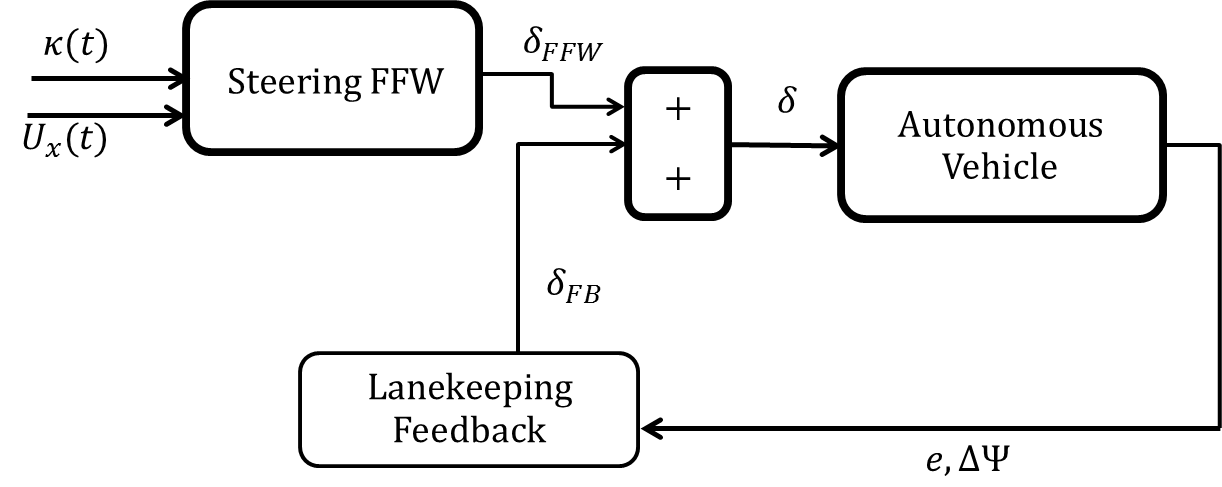
\includegraphics[width=3.25in]{figures/FB_FFW.png}
\caption{Block diagram of feedforward-feedback steering controller.}
\label{fig:controllerBD}
\end{figure}
% % % % % % % end figure % % % % % % %

The desired path curvature for the vehicle to follow is provided to the controller via a separate path planning algorithm \cite{theodosis}. 
Additionally, the velocity profile is obtained from a longitudinal controller that keeps the combined lateral/longitudinal acceleration 
magnitude of the vehicle at a specified value \cite{mickgeneral}.

\vspace{5 mm}
\subsection{Feedforward Steering}

The steering controller uses a feedforward steering command derived from the planar bicycle model (Fig.~\ref{fig:bikeModel}).


\begin{figure}[h]
\centering
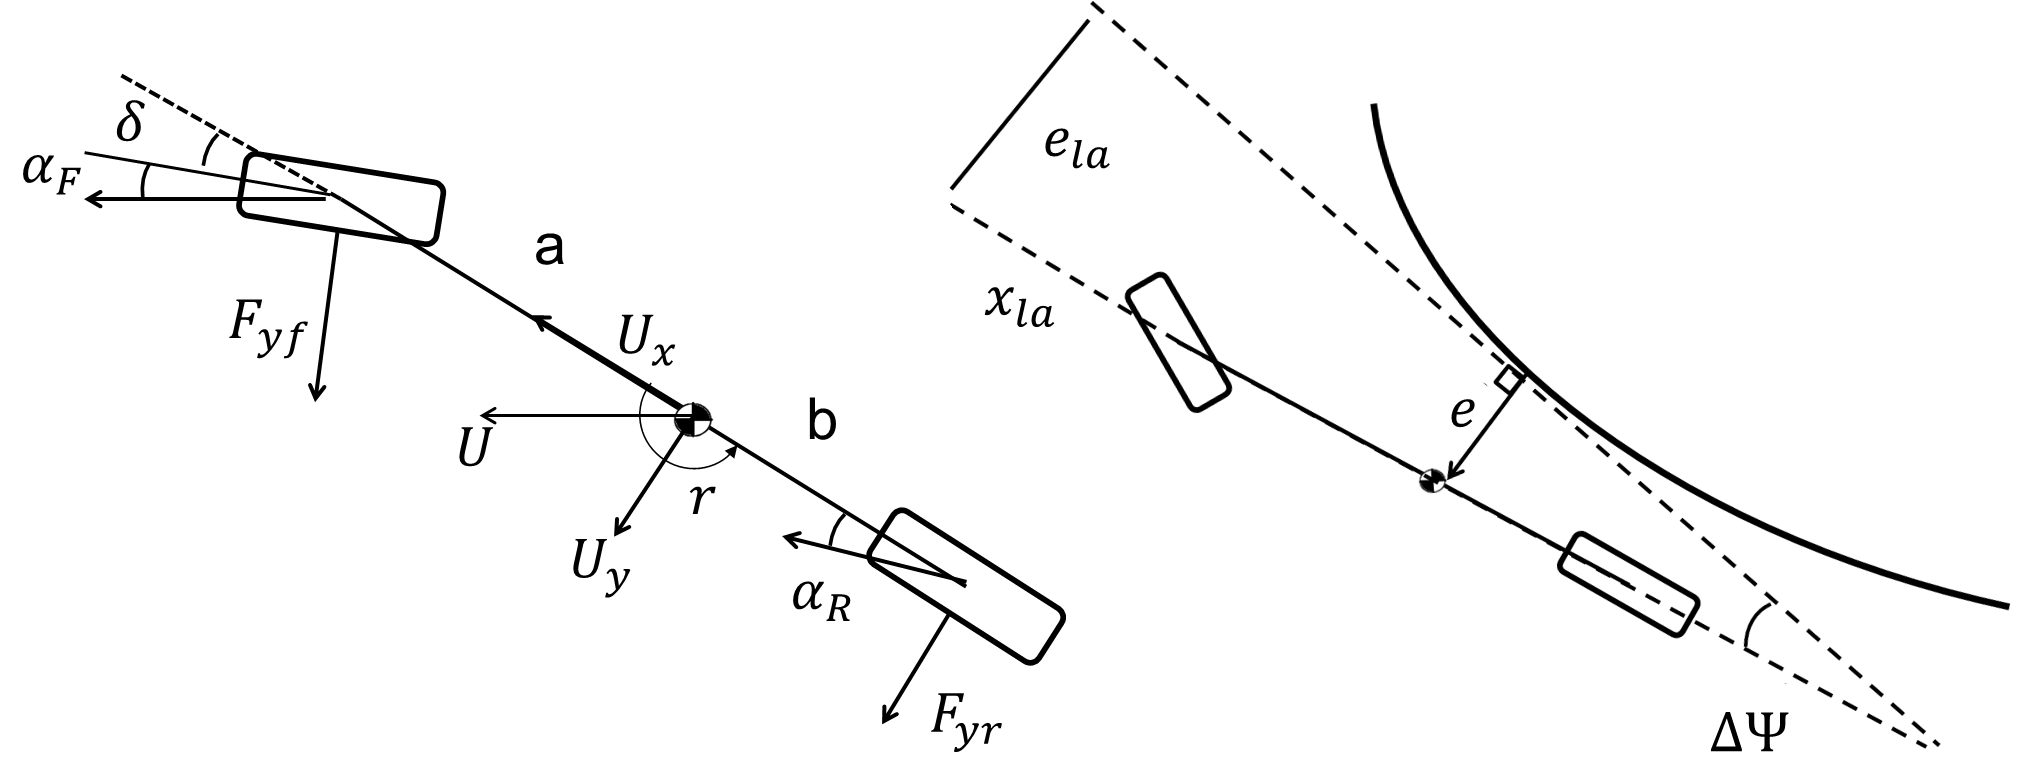
\includegraphics[width=\columnwidth]{figures/BikeModelSchematic.png}
\caption{Schematic of planar bicycle model (left) and error states (right).}
\label{fig:bikeModel}
\end{figure}

Assuming small angles and steady-state cornering, the feedforward steering angle of the vehicle is given from steering geometry as:

\begin{equation}
\label{eqn:ffw}
\delta_{\mathrm{FFW}} = L\kappa - \alpha_\mathrm{f}^\mathrm{FFW}+\alpha_\mathrm{r}^\mathrm{FFW}
\end{equation}
where $L$ is the vehicle length, $\kappa$ is the local path curvature, and $\alpha_\mathrm{f}$ and $\alpha_\mathrm{r}$ are the lumped front and rear tire slip angles respectively. The choice of feedforward 
tire slip angles $\alpha_\mathrm{[f,r]}^\mathrm{FFW}$ depends on the desired feedforward lateral tire forces $F_\mathrm{yf}^\mathrm{FFW}$ and $F_\mathrm{yr}^\mathrm{FFW}$. These forces are chosen to be:

\begin{subequations}
\begin{align}
  F_\mathrm{yf}^\mathrm{FFW} = \frac{mb}{L} U_\mathrm{x}^2\kappa\\
   F_\mathrm{yr}^\mathrm{FFW}=\frac{ma}{L} U_\mathrm{x}^2\kappa
   \end{align}
\end{subequations}
	
An inverted tire model converts the desired tire forces $F_\mathrm{y[f,r]}^\mathrm{FFW}$ into desired tire slip angles $\alpha_\mathrm{[f,r]}^\mathrm{FFW}$. 
To account for saturation of tire force with increasing tire slip magnitude, a single friction coefficient brush Fiala model \cite{Pacejka2012} maps lateral 
tire slip angles into tire force as follows: 

\begin{eqnarray}
\small
	F_\mathrm{y}&=&\begin{cases} -C_{\alpha}\tan\alpha + \frac{C_{\alpha}^2}{3\mu F_\mathrm{z}} |\tan\alpha| \tan\alpha \vspace{2mm} \\ \hspace{4mm}- \frac{C_{\alpha}^3}{27\mu^2F_\mathrm{z}^2}\tan^3\alpha,
\hspace{4mm}  |\alpha| < \arctan{\left(\frac{3\mu F_\mathrm{z}}{C_\alpha}\right)} \\ -\mu F_\mathrm{z}\text{sgn} \ \alpha, \hspace{14mm} \mathrm{otherwise} \end{cases} \nonumber\\
&=&f_{\mathrm{tire}}\left(\alpha\right) \label{eqn:fiala}
\end{eqnarray}
where $\mu$ is the surface coefficient of friction, $F_\mathrm{z}$ is the normal load, and $C_\alpha$ is the tire cornering stiffness. 
These parameters are determined from experimental data taken from a ramp-steer maneuver, as shown in Fig.~\ref{fig:tireCurve}.

\begin{figure}[h]
\centering
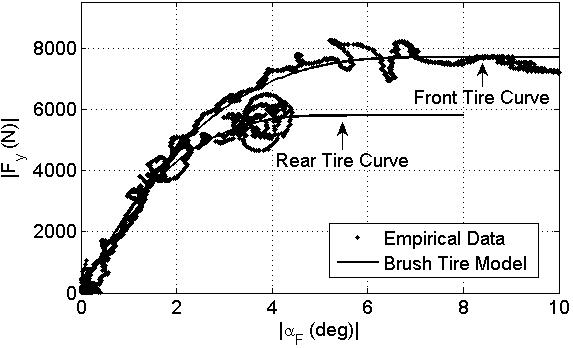
\includegraphics[width=0.98\columnwidth]{figures/FrontRearTireCurves.png}
\caption{Nonlinear tire curves for FFW steering.}
\label{fig:tireCurve}
\end{figure}

\subsection{Experimental Setup}

All vehicle data was collected on an Audi TTS equipped with an electronic power steering motor, active brake booster, and throttle by wire. 
Data was collected over a 1.3 km stretch of paved road (friction coefficient $\mu$ = 1) at Thunderhill Raceway Park in Willows, CA (Fig.~\ref{fig:shelleyPic}).

\begin{figure}[h]
\centering
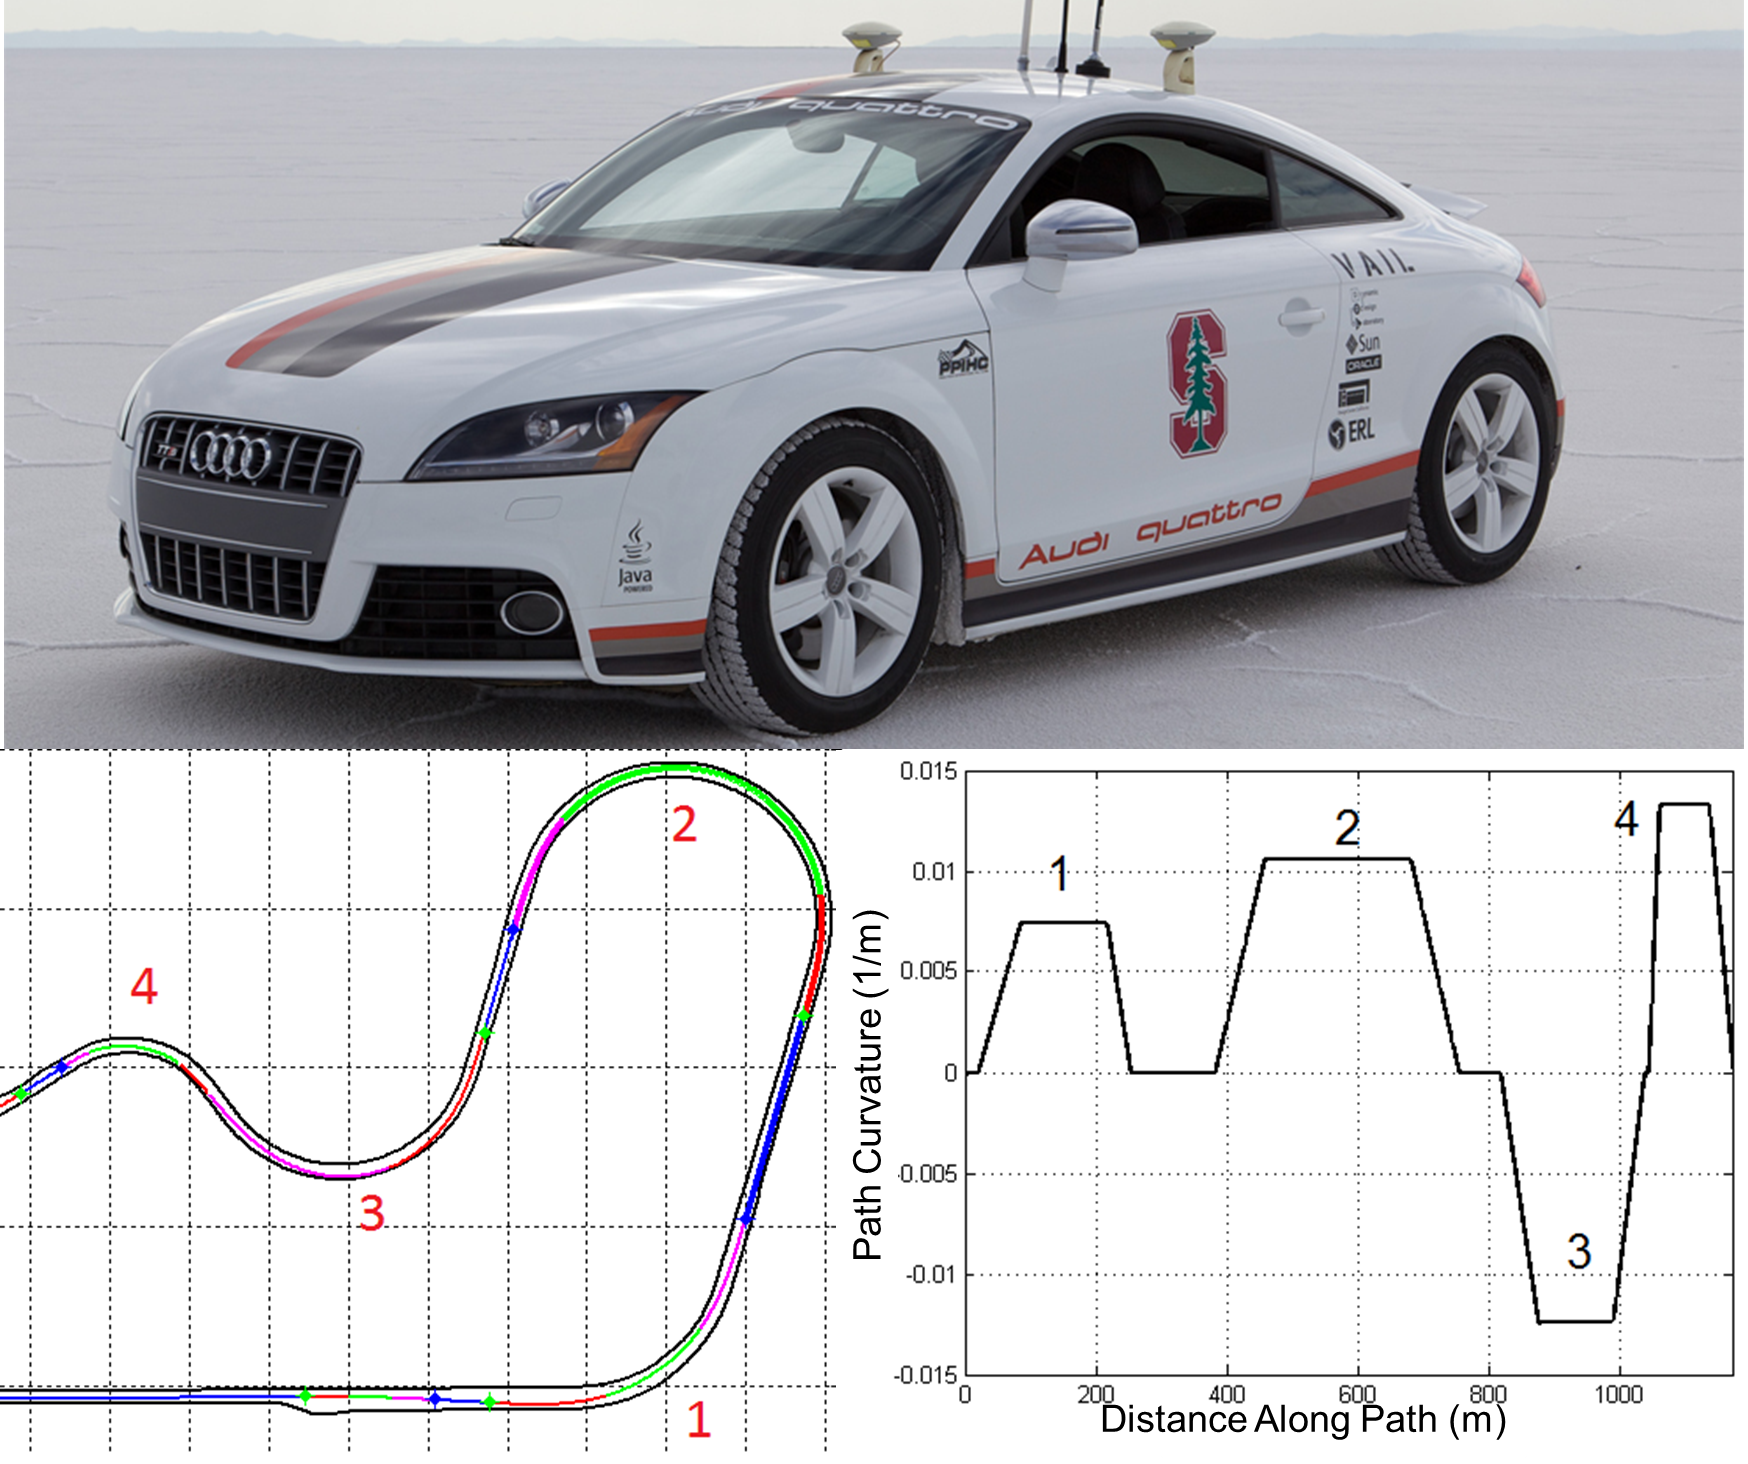
\includegraphics[width=\columnwidth]{figures/experimentInfo.png}
\caption{Top: Audi TTS used for experimental validation. Left: Overhead map of race track. Right: Curvature profile vs. path length of race track segment.}
\label{fig:shelleyPic}
\end{figure}
 
An integrated Differential Global Positioning System (DGPS) and Inertial Measurement Unit (IMU) is used to obtain global vehicle positions and states. 
A map matching algorithm \cite{theodosis} synthesizes information from the INS system to obtain the lateral path deviation
$e$ and vehicle heading error $\Delta\Psi$ in Fig.~\ref{fig:bikeModel}. The controller operates at a 200 Hz sampling rate. Vehicle parameters for the Audi test vehicle are shown in Table \ref{tb:params}.

\begin{table}[h]
\small
\begin{center}
\caption{Vehicle Parameters}\label{tb:params}
\begin{tabular}{lccc}
Parameter & Symbol & Value & Units \\\hline
Vehicle mass & $m$ & 1500 & kg \\
Yaw moment of inertia & $I_z$ & 2250 & $\mathrm{kg \cdot m}^2$\\
Front axle to CG & $a$ & 1.04 & m\\
Rear axle to CG & $b$ & 1.42 & m\\
Front cornering stiffness & $\mathrm{C}_\mathrm{F}$ & 160 & $\mathrm{kN \cdot rad}^{-1}$ \\
Rear cornering stiffness & $\mathrm{C}_\mathrm{R}$ & 180 & $\mathrm{kN \cdot rad}^{-1}$ \\\hline
\end{tabular}
\end{center}
\end{table}

\section{LOOKAHEAD ERROR FEEDBACK}
\label{sec:lookahead}

With the feedforward design complete, the remaining step is to design the feedback controller. One approach to feedback steering is to eliminate a ``lookahead" objective $e_\mathrm{LA}$, which is the vehicle tracking error projected a distance 
$x_\mathrm{LA}$ in front of the vehicle (Fig.~\ref{fig:bikeModel}). The lookahead error is given by 

\begin{equation}
	e_\mathrm{LA}=e+x_\mathrm{LA}\Delta\Psi
\end{equation}
and the resulting feedback control law is

\begin{equation}
	\delta_\mathrm{FB} = -k_\mathrm{P}e_\mathrm{LA}
	\label{eqn:lookahead}
\end{equation}
with proportional gain $k_\mathrm{P}$. The control law (\ref{eqn:lookahead}) is a natural extension of potential field lanekeeping, as described by Rossetter et al. in \cite{rossetter2002}, which also provides heuristics for 
selecting $k_\mathrm{P}$ and $x_\mathrm{LA}$. Desirable stability properties over significant tire saturation levels are demonstrated in \cite{talvala}. 

\vspace{5 mm}
\subsection{Steady-state Error Behavior}

Linear full-state feedback analysis provides useful insight about the steady-state tracking error of the lanekeeping system. From the constant speed 
bicycle model and error state diagram (Fig.~\ref{fig:bikeModel}), linearized equations of motion for the vehicle and error states can be written in state 
space form, with state variable $x= [e \hspace{2 mm} \Delta\Psi \hspace{2 mm} r \hspace{2 mm} \beta]^T$. The linearized control input $\delta$ is defined as follows:

\begin{subequations}
\label{eqn:delta}
\begin{align}
        \delta=\delta_\mathrm{FB}+\delta_\mathrm{FFW} \\
              =[-k_{LK} \hspace{1 mm} -k_{LK} x_{LA} \hspace{3 mm} 0 \hspace{3 mm} 0] x+G_\mathrm{FFW} \kappa
\end{align}
\end{subequations}
 where $G_\mathrm{FFW}= (L+\frac{K_\mathrm{ug} U_\mathrm{x}^2}{g})$ and $K_\mathrm{ug}$ is the vehicle understeer gradient.
Note that $\delta_\mathrm{FB}$ in (\ref{eqn:delta}a) depends on the state variable, and $\delta_\mathrm{FFW}$ depends on the path curvature. Rewriting  
the vehicle state equations of motion using curvature as the input results in:

\begin{equation}
	\label{eqn:sseq}
	\dot{x} = Ax + B\kappa
\end{equation}
where $A$ and $B$ are given by 

\begin{multline}
\label{eqn:Amatrix}
A  =  \\
\left[\begin{smallmatrix}
  0 & U_\mathrm{x} & 0 & U_\mathrm{x} \\ 
  0 & 0 & 1 & 0 \\ 
  \frac{-ak_\mathrm{P} C_\mathrm{F}}{I_\mathrm{z}}  & \frac{-ak_\mathrm{P}x_{LA}C_\mathrm{F}}{I_\mathrm{z}}  & \frac{-(a^2C_\mathrm{F}+b^2C_\mathrm{R})}{U_\mathrm{x}I_\mathrm{z}} & \frac{bC_\mathrm{R} - aC_\mathrm{F}}{I_\mathrm{z}}  \\
  \frac{-k_\mathrm{P}C_\mathrm{F}}{mU_\mathrm{x}}  & \frac{-k_\mathrm{P}x_{LA}C_\mathrm{F}}{mU_\mathrm{x}}  & \frac{bC_\mathrm{r}-aC_\mathrm{f}}{mU_\mathrm{x}^2}-1 & \frac{-(C_\mathrm{F} + C_\mathrm{R})}{mU_\mathrm{x}}
 \end{smallmatrix}\right]
 \end{multline}

\begin{equation}
B =[0 \hspace{2 mm} -U_\mathrm{x} \hspace{3 mm} \frac{a C_\mathrm{F} G_\mathrm{FFW}}{I_\mathrm{z}} \hspace{3 mm}  \frac{C_\mathrm{F} G_\mathrm{FFW}}{mU_\mathrm{x}}]^T
\end {equation}
Fig.~\ref{fig:linError} shows results from using the linear model (\ref{eqn:sseq}) to compute steady-state path
 tracking errors over a range of vehicle speeds, given
 a constant lateral acceleration of $a_y =$ 3 $\mathrm{m/s}^2$. Additionally, results from using the nonlinear 
 tire model (\ref{eqn:fiala}) are plotted for the case where $a_y =$ 7 $\mathrm{m/s}^2$. At low lateral accelerations, when the vehicle
 dynamics are dictated by linear equations of motion, the accumulated steady-state tracking error is small ($<$ .05 m) at highway speeds. However, 
when steering at the limits of handling, Fig.~\ref{fig:linError} shows that the increased sideslip of the vehicle results
 in higher steady-state tracking error, creating challenges for accurate driving. 

\begin{figure}[h]
\centering
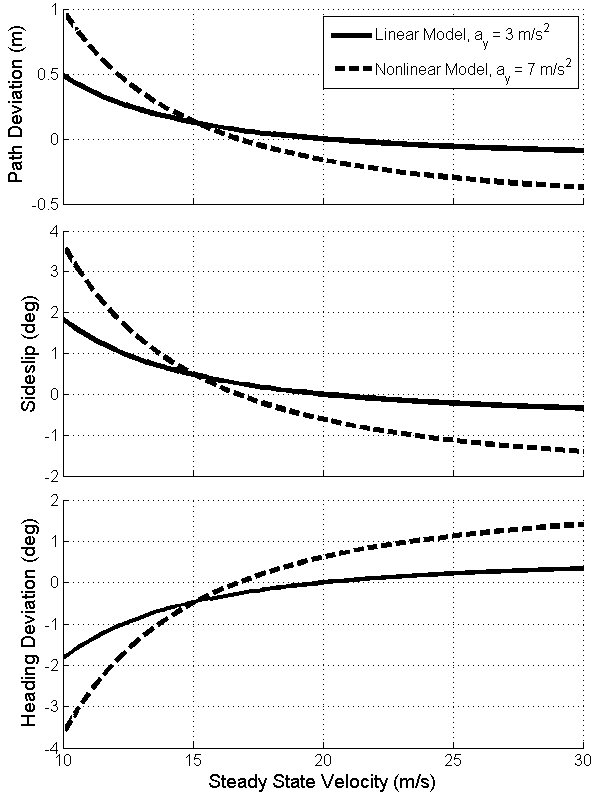
\includegraphics[width=\columnwidth]{figures/LinearErrorPlot.png}
\caption{Steady-state model outputs as a function of vehicle speed. Results are plotted for the linear model, with fixed lateral acceleration $a_y = $ 3 $\mathrm{m/s}^2$, and for the
nonlinear model, with fixed lateral acceleration $a_y = $ 7 $\mathrm{m/s}^2$.}
\label{fig:linError}
\end{figure}

\subsection{Experimental Data}

Fig.~\ref{fig:turn2} depicts experimental data for the setup shown in Fig.~\ref{fig:shelleyPic} with a peak cornering acceleration of 7 $\mathrm{m/s}^2$. The results
mirror the predictions from Fig.~\ref{fig:linError} in that relatively large lateral path deviation $e$ is observed while the vehicle is cornering.

\begin{figure}[h]
\centering
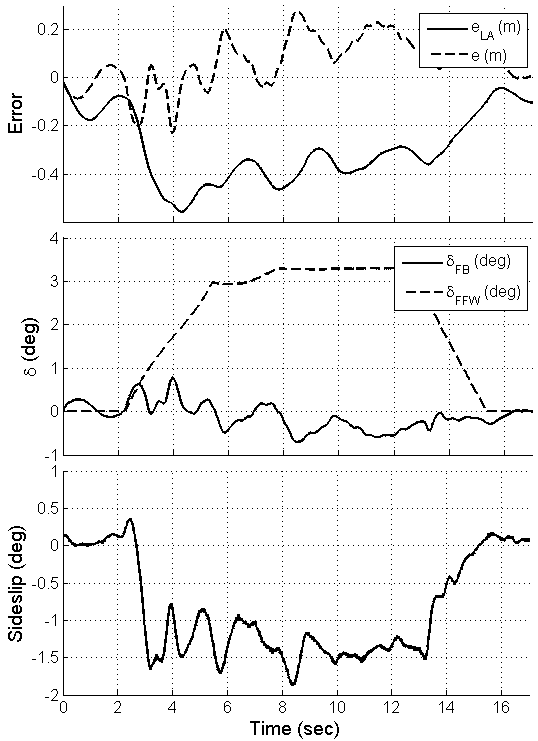
\includegraphics[width=\columnwidth]{figures/Turn2Steering.png}
\caption{Experimental data taken from section 2 of track, with peak lateral acceleration $a_y=$ 7 $\mathrm{m}/\mathrm{s}^2$. }
\label{fig:turn2}
\end{figure}

A qualitative explanation for this steady-state error is shown in Fig.~\ref{fig:SSerror}. Because the steering controller acts to eliminate a weighted
sum of heading error $\Delta\Psi$ and lateral path deviation $e$, the lookahead feedback is successful in
minimizing the desired metric $e_\mathrm{LA}$ at the projected distance $x_\mathrm{LA}$ in front of the vehicle. However, this still allows for steady state equilibria where
values of $e$ and $\Delta\Psi$ themselves are nonzero.  


\begin{figure}[h]
\centering
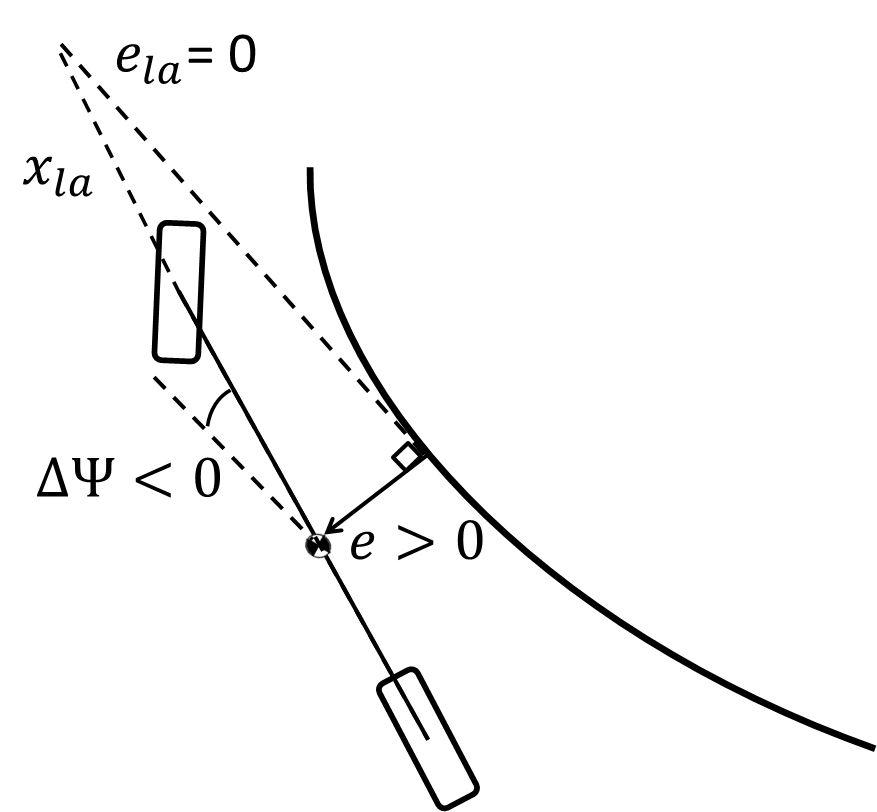
\includegraphics[width=0.6\columnwidth]{figures/SSerror.png}
\caption{Steady-state cornering where vehicle has lateral error but no lookahead error.  }
\label{fig:SSerror}
\end{figure}

\vspace{6 mm}




% % % % % % % end figure % % % % % % %

%=======================================================================
\section{VELOCITY VECTOR FEEDBACK}
\label{sec:vvfb}

An interesting observation from Fig.~\ref{fig:linError} is that the steady-state path deviation
 is zero at a vehicle speed of around $U_\mathrm{x}$=20 m/s for the linear model and $U_\mathrm{x}$=17 m/s for the nonlinear model. 
 At these speeds, the steady-state vehicle sideslip is predicted to be zero as well, 
and the vehicle heading $\Psi$ naturally becomes tangent to the desired path heading. 
\begin{figure}[h]
\centering
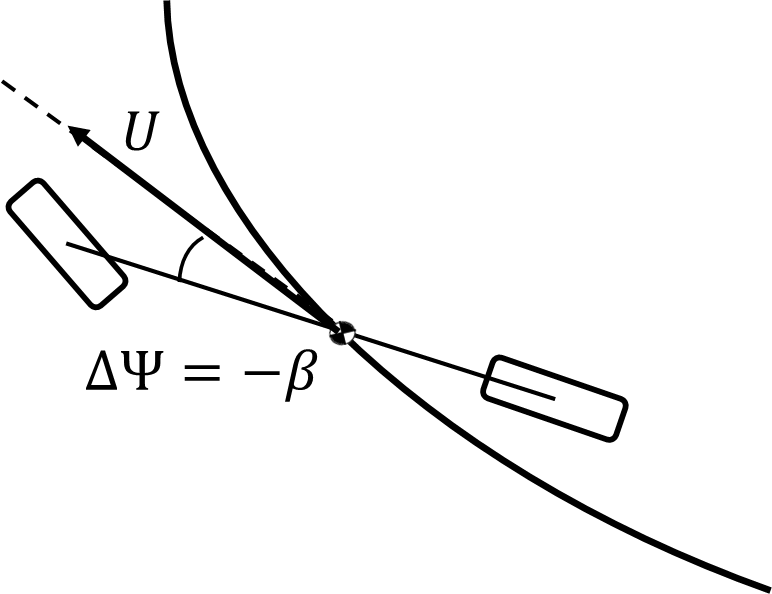
\includegraphics[width=0.5\columnwidth]{figures/LookaheadWithSideslip.png}
\caption{Schematic of vehicle velocity feedback.}
\label{fig:lawithsideslip}
\end{figure}

This observation motivates a second form of lanekeeping feedback where the feedback aims to keep the 
vehicle velocity vector $U$ tangent to the desired path (Fig.~\ref{fig:lawithsideslip}). Since
 $U=\Psi+\beta$, the resulting control law is:
 
 
\begin{subequations}
\label{eqn:vveq}
\begin{align}
        \delta_\mathrm{FB} & = -k_\mathrm{P} (e+x_\mathrm{LA}  \sin⁡(U-\Psi_\mathrm{r} ) ) \\
                           & =  -k_\mathrm{P} (e+x_\mathrm{LA} (\Psi+\beta-\Psi_\mathrm{r} )) \\
						   & = -k_\mathrm{P}(e+x_{LA}(\Delta\Psi+\beta))
\end{align}
\end{subequations}
 where $\Psi_\mathrm{r}$ is the heading of the desired vehicle path at a given point. The modified control law can be modeled by reformulating (\ref{eqn:Amatrix}) as:
 
\begin{multline}
\label{eqn:Amatrix2}
A  =  \\
 \left[\begin{smallmatrix}
  0 & U_\mathrm{x} & 0 & U_\mathrm{x} \\
  0 & 0 & 1 & 0 \\
  \frac{-ak_\mathrm{P} C_\mathrm{F}}{I_\mathrm{z}}  & \frac{-ak_\mathrm{P}x_{LA}C_\mathrm{F}}{I_\mathrm{z}}  & \frac{-a^2C_\mathrm{F}-b^2C_\mathrm{R}}{U_\mathrm{x}I_\mathrm{z}} & \frac{bC_\mathrm{R} - aC_\mathrm{F}(1-ak_\mathrm{P}x_\mathrm{LA}) }{I_\mathrm{z}}  \\
  \frac{-k_\mathrm{P}C_\mathrm{F}}{mU_\mathrm{x}}  & \frac{-k_\mathrm{P}x_{LA}C_\mathrm{F}}{mU_\mathrm{x}}  & \frac{-aC_\mathrm{f}-bC_\mathrm{r}}{mU_\mathrm{x}^2}-1 & \frac{-(C_\mathrm{F}(1+k_\mathrm{P}x_\mathrm{LA}) + C_\mathrm{R})}{mU_\mathrm{x}}
 \end{smallmatrix}\right]
 \end{multline}
 
Note that (\ref{eqn:Amatrix2}) is equal to (\ref{eqn:Amatrix}) with the exception of the last column. Fig.~\ref{fig:linError2}
shows the resulting steady-state behavior, and indicates that lateral error $e$ settles to
zero for all velocities. 

\begin{figure}[h]
\centering
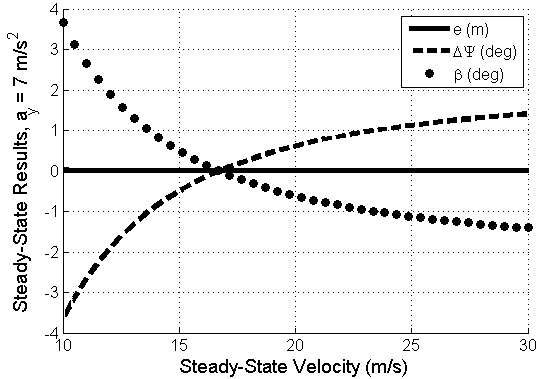
\includegraphics[width=\columnwidth]{figures/LinearErrorPlotBeta.png}
\caption{Steady-state simulation results for velocity vector feedback, using the nonlinear vehicle model with fixed lateral acceleration of 7 $\mathrm{m/s^2}$.}
\label{fig:linError2}
\end{figure}

However, the disadvantage of directly adding vehicle sideslip 
into the feedback control is reduced stability margins. One method of observing the relative stability benefits of lookahead feedback is to compute the eigenvalues of (\ref{eqn:Amatrix2}) and (\ref{eqn:Amatrix}) for different
values of the lookahead distance $x_\mathrm{LA}$ and different vehicle understeer configurations. Fig.~\ref{fig:VcrPlot} shows the critical speed $V_\mathrm{cr}$, beyond which the closed loop steering system
becomes unstable, for neutral, understeering, and oversteering configurations as a function of $x_\mathrm{LA}$. For an understeering vehicle, lookahead feedback is always stable as long
as the lookahead point $x_\mathrm{LA}$ is above a certain critical value (a conclusion derived in \cite{rossetter2002}). Even in situations where the vehicle is in a 
neutral steer or oversteer configuration, the critical speed for closed loop stability increases rapidly with lookahead distance. A different trend is present for the velocity vector
feedback. Fig.~\ref{fig:VcrPlot} shows that the critical speeds for stability increase very slowly as a function of lookahead distance.  

\begin{figure}[h]
\centering
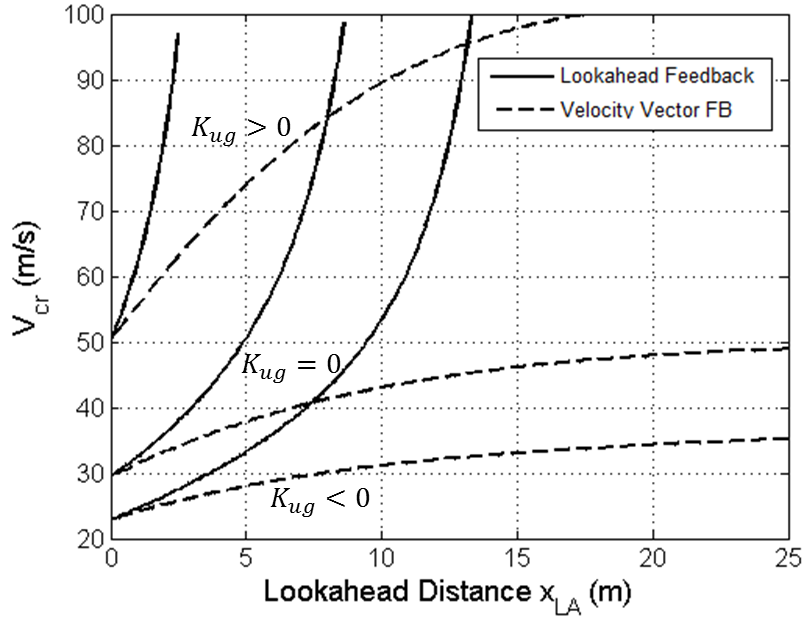
\includegraphics[width=\columnwidth]{figures/VcrPlot.png}
\caption{Maximum speed for closed loop stability for lookahead feedback and velocity vector feedback, based on the linear vehicle model.}
\label{fig:VcrPlot}
\end{figure}

\section{VELOCITY VECTOR TRACKING WITH STEADY-STATE SIDESLIP}
\label{sec:ssbeta}
 
 Given the tradeoff between path tracking and stability with the velocity vector feedback, a promising approach
 is to replace vehicle sideslip  $\beta$ in (\ref{eqn:vveq}) with the predicted steady-state sideslip value $\beta_\mathrm{ss}$ 
 for a given vehicle speed and curvature. 

The rear tire slip for a fixed track vehicle, assuming small angles, is given by 
\begin{equation}
\alpha_\mathrm{r} = \beta - \frac{br}{U_\mathrm{x}}
\end{equation} 

Where $r$ is the vehicle yaw rate. At steady-state, $\alpha_\mathrm{r}=\alpha_\mathrm{r}^\mathrm{FFW}$ from (\ref{eqn:ffw}) and $r_\mathrm{ss}=\kappa U_\mathrm{x}$, yielding the following feedback control law:

\begin{equation}
\delta_\mathrm{FB}=-k_\mathrm{P} (e+x_\mathrm{LA} (\Delta\Psi+\beta_\mathrm{ss}))
\end{equation}

\begin{equation}
\beta_\mathrm{ss} = \alpha_\mathrm{r}^\mathrm{FFW} + b\kappa
\end{equation}

The effect of this change is to remove the feedback control law's explicit dependence on real-time sideslip information.
The state matrix equation $A$ for the closed loop system dynamics (\ref{eqn:sseq}) is now once again given by (\ref{eqn:Amatrix}), which was shown to have desirable stability
properties as a function of $K_\mathrm{ug}$ and $x_\mathrm{LA}$ (Fig.~\ref{fig:VcrPlot}). The sideslip now affects the vehicle path tracking dynamics through the feedforward path, and the
$B$ matrix now becomes: 

\begin{equation}
\label{eqn:newB}
\small
B =[0 \hspace{2 mm} -U_\mathrm{x} \hspace{3 mm} \frac{a C_\mathrm{F} (G_\mathrm{FFW}+G_\beta)}{I_\mathrm{z}} \hspace{3 mm}  \frac{C_\mathrm{F} (G_\mathrm{FFW}+G_\beta)}{mU_\mathrm{x}}]^T
\end {equation}

\begin{equation}
G_\beta = U_\mathrm{x}^2\frac{ma}{L}\frac{k_\mathrm{P}x_\mathrm{LA}}{C_\mathrm{R}}
\end{equation}

 

\begin{figure}[h]
\centering
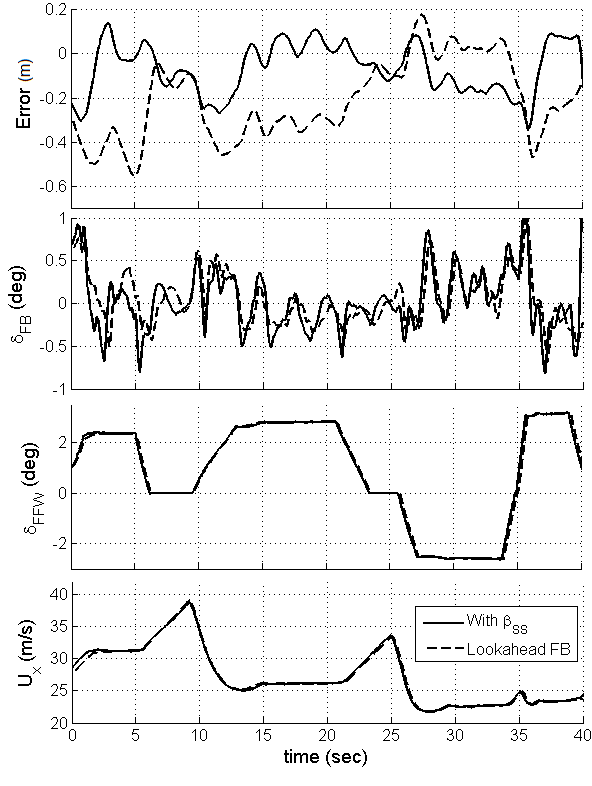
\includegraphics[width=\columnwidth]{figures/betaCompensation.png}
\caption{Experimental data with combined acceleration magnitude 7 $\mathrm{m/s^2}$ over 1.3 km stretch of Thunderhill Raceway Park.}
\label{fig:betaComparison}
\end{figure}

Fig.~\ref{fig:betaComparison} shows experimental data taken over the entire 1.3 km stretch of racetrack (Fig.~\ref{fig:shelleyPic}), using the lookahead steering controller and the
velocity vector tracking with steady-state sideslip. The same longitudinal controller is used for both cases, with 
 longitudinal dynamics applied to brake into the entry of turns and accelerate out of turn exits. The braking and cornering are applied in a
 manner such that peak deceleration is -7 $\mathrm{m/s^2}$ and peak cornering acceleration is 7 $\mathrm{m/s^2}$.

The results show that lateral path deviation $e$ is substantially reduced when incorporating steady-state sideslip in the feedforward control law, with the exception of the 
time period between 27 and 35 seconds. Since the steering controller now accounts for the vehicle sideslip in the feedforward term, steady-state path tracking errors can exist in the presence of unmodelled plant dynamics or
 incorrectly estimated vehicle parameters. This is seen in the experimental data of Fig.~\ref{fig:betaComparison} from $t$ = 27-35 seconds, where the car was driving on a banked portion of the track.  



%=======================================================================
\section{CONCLUSION AND FUTURE WORK}

This paper describes the design of a feedforward-feedback controller capable of path tracking at the limits of handling. Desirable path tracking behavior occurs when the vehicle sideslip is aligned
with the desired path heading. However, directly incorporating this behavior using steering feedback results in a closed loop controller with poor stability margins. 
A better approach for combined path tracking and stability is to align the steady-state vehicle sideslip with the desired path heading through the feedforward steering command. 
This enables improved path tracking while maintaining the robust stability properties of traditional lookahead control. One potential drawback is that this feedforward approach is sensitive to vehicle model uncertainty, especially at the physical
limits of handling where transient dynamics become prevalent. Future work will seek to use methods such as iterative learning control to eliminate undesirable transient dynamics. \\

%=======================================================================
\bigskip
\bibliography{Bibliography}  % bib file to produce the bibliography
\bibliographystyle{asmems4}

\bigskip
\noindent\textbf{ACKNOWLEDGEMENTS}\\
\\
This research is supported by the National Science Foundation Graduate Research Fellowship Program (GRFP). 
The authors would also like to thank the members of the Dynamic Design Lab at Stanford University and the Audi Electronics Research Lab.

\end{document}